\subsubsection{Biochemistry - Methyltransferases}
\index{Jeltsch, Albert}

\paragraph{Research Team}
%
Albert Jeltsch (Professor),
Sandra Becker (Technician),
Sanjay Chahar (PhD Student),
Arunkumar Dhayalan (PhD Student),
Renata Jurkowska (PhD Student),
Tomek Jurkowski (PhD Student),
Heike Laser (Postdoc),
Kirsten Liebert (Postdoc),
Sergei Ragozin (Postdoc),
Philipp Rathert (PhD Student),
Christian Rohde (PhD Student),
Martina Schlickenrieder (PhD Student),
Maike Schwerdtfeger (Lab Technician),
Yinying Zhang (PhD Student)\\

DNA methylation is an important regulator for gene expression in mammals. Methylation of human DNA at CG sites is a central trigger for cellular differentiation and gene regulation. In bacteria, DNA methylation is involved in various processes including DNA repair, gene regulation, phase variation and pathogenicity. We study the DNA recognition, structure and enzymatic mechanism of prokaryotic DNA methyltransferases from E.coli, phages, Salmonella and other bacteria with the aim to develop specific inhibitors for these enzymes that are potentially active as antibiotics. Mammalian enzymes are studied to understand the process of generation and preservation of methylation patterns in human cells. We are involved in approaches to analyze the methylation pattern of human DNA. The results will allow understanding differentiation and gene regulation at better level which is a pre- requisite for successful application of cloning procedures for organ replacement in the future.


\paragraph{Highlights}

The specific interaction of proteins with DNA is a fundamental process in the regulation of gene expression in all organisms. In collaboration with the group of  X. Cheng (Atlanta, GR) we have solved the structure of the EcoDam DNA methyltransferase and elucidated how this enzyme specifically recognizes its GATC target site on DNA. The structural analysis revealed that the enzyme forms four specific interactions to the bases of the DNA, the importance of these contacts was confirmed by biochemical studies with enzyme variants after removal of some of the important residues. One striking result of that study was that the process of contacting the DNA resembles closing of a zipper in which the interactions on one site of the target are formed earlier while others follow in an ordered pathway. Changing of the amino acid residues that contact the DNA allowed to modify the DNA interaction of the enzyme and create enzyme variant with new DNA recognition specificities. These results shed light on the principles of protein/DNA interactions. Furthermore, the detailed structural and functional knowledge about the dam DNA methyltransferase might enable us in the future to design new types of antibiotics which inactivate this protein, which has been shown to be important for pathogenicity in several important human pathogens.

\begin{figure}[ht]
  \begin{center}
   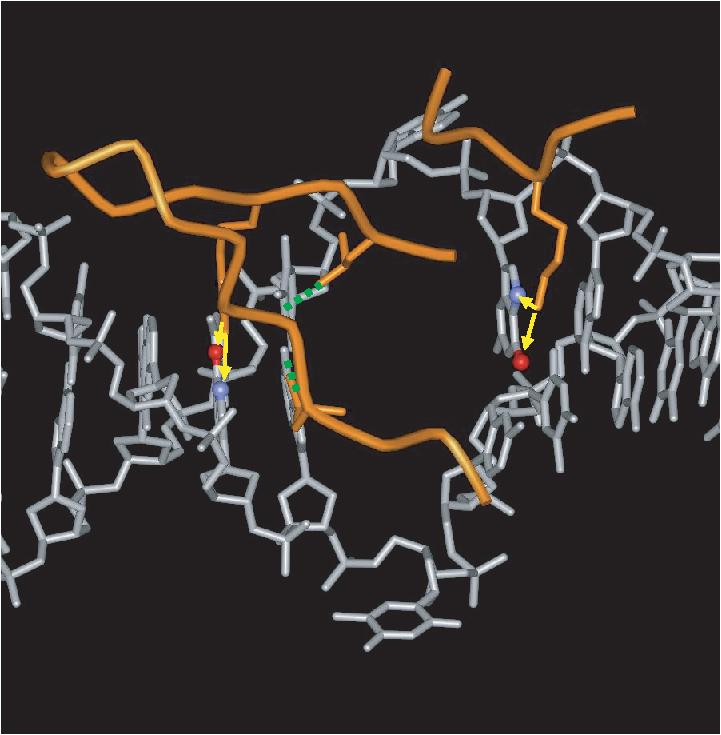
\includegraphics[width=\hsize]{Jeltsch/Fig_Jeltsch1_2006.pdf}
    \mycaption{Structure of the Ecodam Methyltransferase in complex with specific DNA.}\label{Fig_Jeltsch1_2006.pdf}
   \end{center}
\end{figure}

In a second project, we study the function of mammalian DNA methyltransferases. In mammals, the DNA methylation pattern is copied during each round of DNA replication. In cooperation with R. Reinhardt (Berlin, Germany) we have studied the mechanism and specificity of the Dnmt1 enzyme which has a central role in copying the pattern of DNA methylation after replication and thereby mediates epigenetic inheritance of the patterns of gene expression in various cell types. Using long hemimethylated DNA substrates that carry defined methylation patterns and bisulfite analysis of the methylation reaction products, we show that the enzyme has a 15 fold preference for hemimethylated CG sites. Dnmt1 moves along the DNA in a random walk methylating hemimethylated substrates with high processivity ($>$50 sites are visited on average which corresponds to linear diffusion over 6000 base pairs). These properties are jmportant for the physiological function of Dnmt1.\newline \newline Albert Jeltsch is also involved in ``Enzyme Design''.

\myparagraph{Collaborations}
%
Bremen Area Collaborations:
\begin{enumerate}
%
\item {\sl International University Bremen} \\ Prof. K. Brix \\ Confocal cell imaging
 \\ Prof. G. Mushkelishvili \\ AFM of DNA methyltransferases
 \\ Prof. W. Nau \\ Investigation of Peptide Dynamics
\\ Prof. S. Springer \\ Rapid Kinetics
\\ Dr. H. Stamerjohanns \\ Data analysis and web programming
 \\ Prof. M. Ullrich \\ Mass spectrometry
 \\ Dr. C. Voelcker-Rehage \\ Genkotyping participants of the JC aging study
 \\ Prof. M. Winterhalter \\ Dynamic light scattering
 \\ Prof. M. Zacharias \\ Simulation of enzyme dynamics

\end{enumerate}
National \& International Collaborations:
\begin{enumerate}
\item {\sl University of Texas, Department of Carcinogenesis, Smithville, Texas, USA} \\ Prof. M.T. Bedford \\ Peptide interaction of DNA methyltransferases
\item {\sl Emory University Atlanta, Department of Medicine, GA, USA} \\ Prof. X. Cheng \\ X-ray crystallography and inhibitor design of DNA methyltransferases
\item {\sl Universit�t Halle} \\ Prof. R. Dammann \\ Expression of Dnmt1 in cells
\item {\sl University of Edinburgh, Edinburgh, UK} \\ Prof. D.T.F. Dryden \\ Time resolved fluorescence spectroscopy with DNA methyltransferases
\item {\sl Laboratory of Cancer Epigenetics, Faculty of Medicine, Free University of Brussels, Brussels, Belgium} \\ Prof. F. Fuks \\Phosphorylation of DNA methyltransferases
\item {\sl DKFZ, Heidelberg} \\ Prof. I. Grummt \\ Regulation of DNA methyltransferases in cells
\item {\sl Hungarian Academy of Science, Szeged, HU} \\ Prof.  A. Kiss \\ Expression and Design of the M.SssI DNA methyltransferase
\item {\sl Department of Biochemistry and Molecular Biology, University of Shaanxi, China} \\ Dr. F. Li \\Targeted methylation of DNA in cells
\item {\sl DKFZ, Heidelberg} \\ Dr. F. Lyko \\ Expression and characterisation of Dnmt2
\item {\sl University of Groningen, Groningen, The Netherlands} \\ Dr. P. McLaughlin\\ Targeted methylation of DNA in cells
\item {\sl National Cancer Institute, Frederick, MD, USA} \\ Prof. K. Muegge \\ Regulation of Dnmt3a in cells
\item {\sl Institut f�r Genetik, Universit�t Kassel} \\Prof. W. Nellen \\ Expression and characterisation of Dnmt2
\item {\sl The Wellcome Trust Biocentre, University of Dundee, Dundee, UK} \\ Prof. T. Owen-Hughes \\ Preparation of nucleosomal DNA
\item {\sl MRC, Cambridge, UK} \\ Dr. M. Papworth\\ Targeted methylation of DNA in cells
\item {\sl Leibnitz Institute for Age Research, Jena} \\ Dr. M. Platzer \\ High troughput DNA Sequencing
\item {\sl Justus-Liebig Universit�t Giessen} \\ Prof. A. Pingoud \\ Targeted DNA cleavage
\item {\sl MPI f�r Molekulare  Genetik, Berlin }\\ Dr. R. Reinhardt \\ High troughput DNA sequencing
\item {\sl CNRS/University of Rennes 1 Joint Unit, Rennes, France} \\ Dr. G. Salbert \\ Enzymology of Dnmt3a
\item {\sl MHH, Hannover \\ Prof. C. Urbanke} \\ Analytical Ultracentrifugation
\item {\sl Universit�t Saarbr�cken} \\ Prof. J. Walter \\Human Methylome analysis
\item {\sl Chinese Academy of Sciences, Shanghai, China} \\ Prof. G. Xu \\ Biologcial role of Dnmt3a
\end{enumerate}

\paragraph{Organization}
%
\begin{enumerate}
\item {Member of the editorial board of BMC Biochemsitry}
\end{enumerate}

 \paragraph{Grants}
\begin{enumerate}
\item Funded by BMBF, Biofuture \emph{Development of programmable
DNA methyltransferases for biotechnological applications },
(August 2003 - Dezember 2007)
 \item
Funded by BMBF,  BioChancePlus \emph{Amplification of DNA with
preservation of the methylation state }, (May 2004 - April 2007)

\item Funded by BMBF,  SMP Epigenetics \emph{Analysis of the DNA
methylation pattern of genes on Chromosome 21 } , (May 2005 -
April 2007)

\item Funded by NIH (USA), \emph{Histone Lysine Methylation:
structures and functions},  (October 2006 - September 2011)

\item Funded by DFG,  priority program SPP1070 \emph{Directed
evolution of DNA methyltransferases}, JE252/5-1 and 5-2,
 (September 2004 - May 2007) (JE252/5-1), (December 2006 -
December 2008) (JE252/5-2)

\item Funded by DFG,  priority program SPP1129 \emph{Biochemistry
and biological function of mammalian Dnmt1 and Dnmt2}, JE252/4-2
and 4-3, (December 2005 - November 2007) (JE252/4-2), (October
2006 - December 2008) (JE252/4-3)

\item Funded by DFG, \emph{Enzymology, structure and DNA
recognition of the E. coli dam DNA methyltransferase}, JE252/2-6,
(October 2005 - December 2008)




\end{enumerate}

\paragraph{Other Support Grants}
\begin{enumerate}
\item {JE252/2-5 (DFG) ``Enzymology, structure and DNA recognition of the E. coli dam DNA methyltransferase'' at University of Gie\ss en}
\item {HBFG 066/7-1 (DFG) ``Purchase of a MALDI TOF mass spectrometer''}
\end{enumerate}


\paragraph{Patents}
\begin{enumerate}
\item {Patent application: Pingoud, Jeltsch, Eisenschmidt: Hochspezifisch mit DNA interagierende Enzym-Konjugate. EPA 2005/009028 (pending)}
\item {Cheng, Horton, Yang, Calman, Zhang, Jeltsch, Hattmann ``Small Molecule Inhibitors of Bacterial Dam DNA Methyltransferases'', PCT Patent Application No. PCT/US 05/44277, 2006 (pending)}
\end{enumerate}


\paragraph{Awards, Prices}
\begin{enumerate}
\item {Elected as vice-president of the DNA Methylation Society (New Orleans, LO)}
\end{enumerate}


\nocite{Jeltsch1,Jeltsch2,Jeltsch3,Jeltsch4,Jeltsch5,Jeltsch6,Jeltsch7,Jeltsch8,Jeltsch9,Jeltsch10}
